%%%%%%%%%%%%%%%%%%%%%%%%%%%%%%%%%%%%%%%%%%%%%%%%%%%%%%%%%%%

\chapter{Modello del sistema - gruppo 2 - notifiche}
\label{ref:modSistemaGruppo2-notifiche}

\section{Attori}

<Gli attori di Notifiche sono in comune agli altri gruppi>.

\section{Scenari}

\subsection{Apertura finestra di prenotazione per l’appello d’esame}

Il sistema invia una notifica push allo studente Angelo Gino Varrati, identificato per mezzo di matricola 123456, in concomitanza con l’apertura della finestra di prenotazione dell’esame di “Ingegneria del Software” del Prof. Fausto Fasano, in quanto ancora da sostenere e presente all’interno della propria carriera.

\subsection{Chiusura finestra di prenotazione per l’appello d’esame}

Il sistema invia una notifica push alla studentessa Giuseppina Mazzocco, identificata per mezzo di matricola 789101, poco prima della chiusura della finestra di prenotazione all’esame di “Ingegneria del Software” del Prof. Fausto Fasano, in quanto ancora da sostenere e presente all’interno della propria carriera.

\subsection{Verbalizzazione esame}

Il sistema invia una notifica push alla studentessa Martina Buro, identificata per mezzo di matricola 234567, in occasione della verbalizzazione dell’esame di “Ingegneria del Software” del Prof. Fausto Fasano, sostenuto in data 28/02/2019 riportando votazione pari a 28.

\subsection{Avviso tasse}

All’apertura del periodo di pagamento di un importo di tasse universitarie, tale evento verrà notificato all’utente per mezzo di una notifica push.

\subsection{Sospensione lezione}

Il sistema invia una notifica push allo studente Angelo Gino Varrati, identificato per mezzo di matricola 123456, in occasione della sospensione della lezione di “Ingegneria del Software” del Prof. Fausto Fasano prevista per il giorno 19/03/2019.

\section{Casi d'uso}

\subsection{Gestione notifiche}

Il caso d'uso \emph{Gestione notifiche} è identico per tutte le notifiche, ciò che cambia è unicamente il contenuto della modifica. Vedi Tabella~\vref{tab:caso-duso-gestione-notifiche}.

\begin{table}
%\normalsize % Dimensione testo normale
\small % Dimensione testo piccola
%\footnotesize % Dimensione testo piccolissima
%\scriptsize % Dimensione del testo ulteriormente più piccola
\caption{Tabella caso d'uso - Gestione notifiche} % Didascalia tabella
\label{tab:caso-duso-gestione-notifiche} % Etichetta per riferimenti incrociati
\begin{tabular}{| p{\useCaseLeft} | p{\useCaseNum} | p{\useCaseTwoCol} | p{\useCaseTwoCol} |}
	\hline
	\textbf{Nome caso d'uso} & \multicolumn{3}{p{\useCaseMulticol} |}{\textbf{Gestione notifiche}} \\
	\hline
	\textbf{Attori partecipanti} & \multicolumn{3}{p{\useCaseMulticol} |}{Inizializzato da Firebase. Partecipa Studente.} \\
	\hline
	\textbf{Condizioni d'ingresso} & \multicolumn{3}{p{\useCaseMulticol} |}{Connessione ad Internet.} \\
	\hline
	\textbf{Flusso degli eventi} & \textbf{\#} & \textbf{Studente} & \textbf{Firebase} \\
	\hline
	\textbf{} & \textbf{1} & \textbf{} & Invia una notifica. \\
	\hline
	\textbf{} & \textbf{2} & Riceve la notifica. & \textbf{} \\
	\hline
	\textbf{Eccezioni} & \multicolumn{3}{p{\useCaseMulticol} |}{Lo Studente ha disabilitato la ricezione delle notifiche.} \\
	\hline
	\textbf{Condizioni d'uscita} & \multicolumn{3}{p{\useCaseMulticol} |}{Lo studente visualizza la notifica.} \\
	\hline
\end{tabular}
\end{table}

\section{Diagrammi dei casi d'uso}

Vedi Figura~\vref{fig:diagr-casi-duso-notifiche}.

\begin{figure}
	\centering
	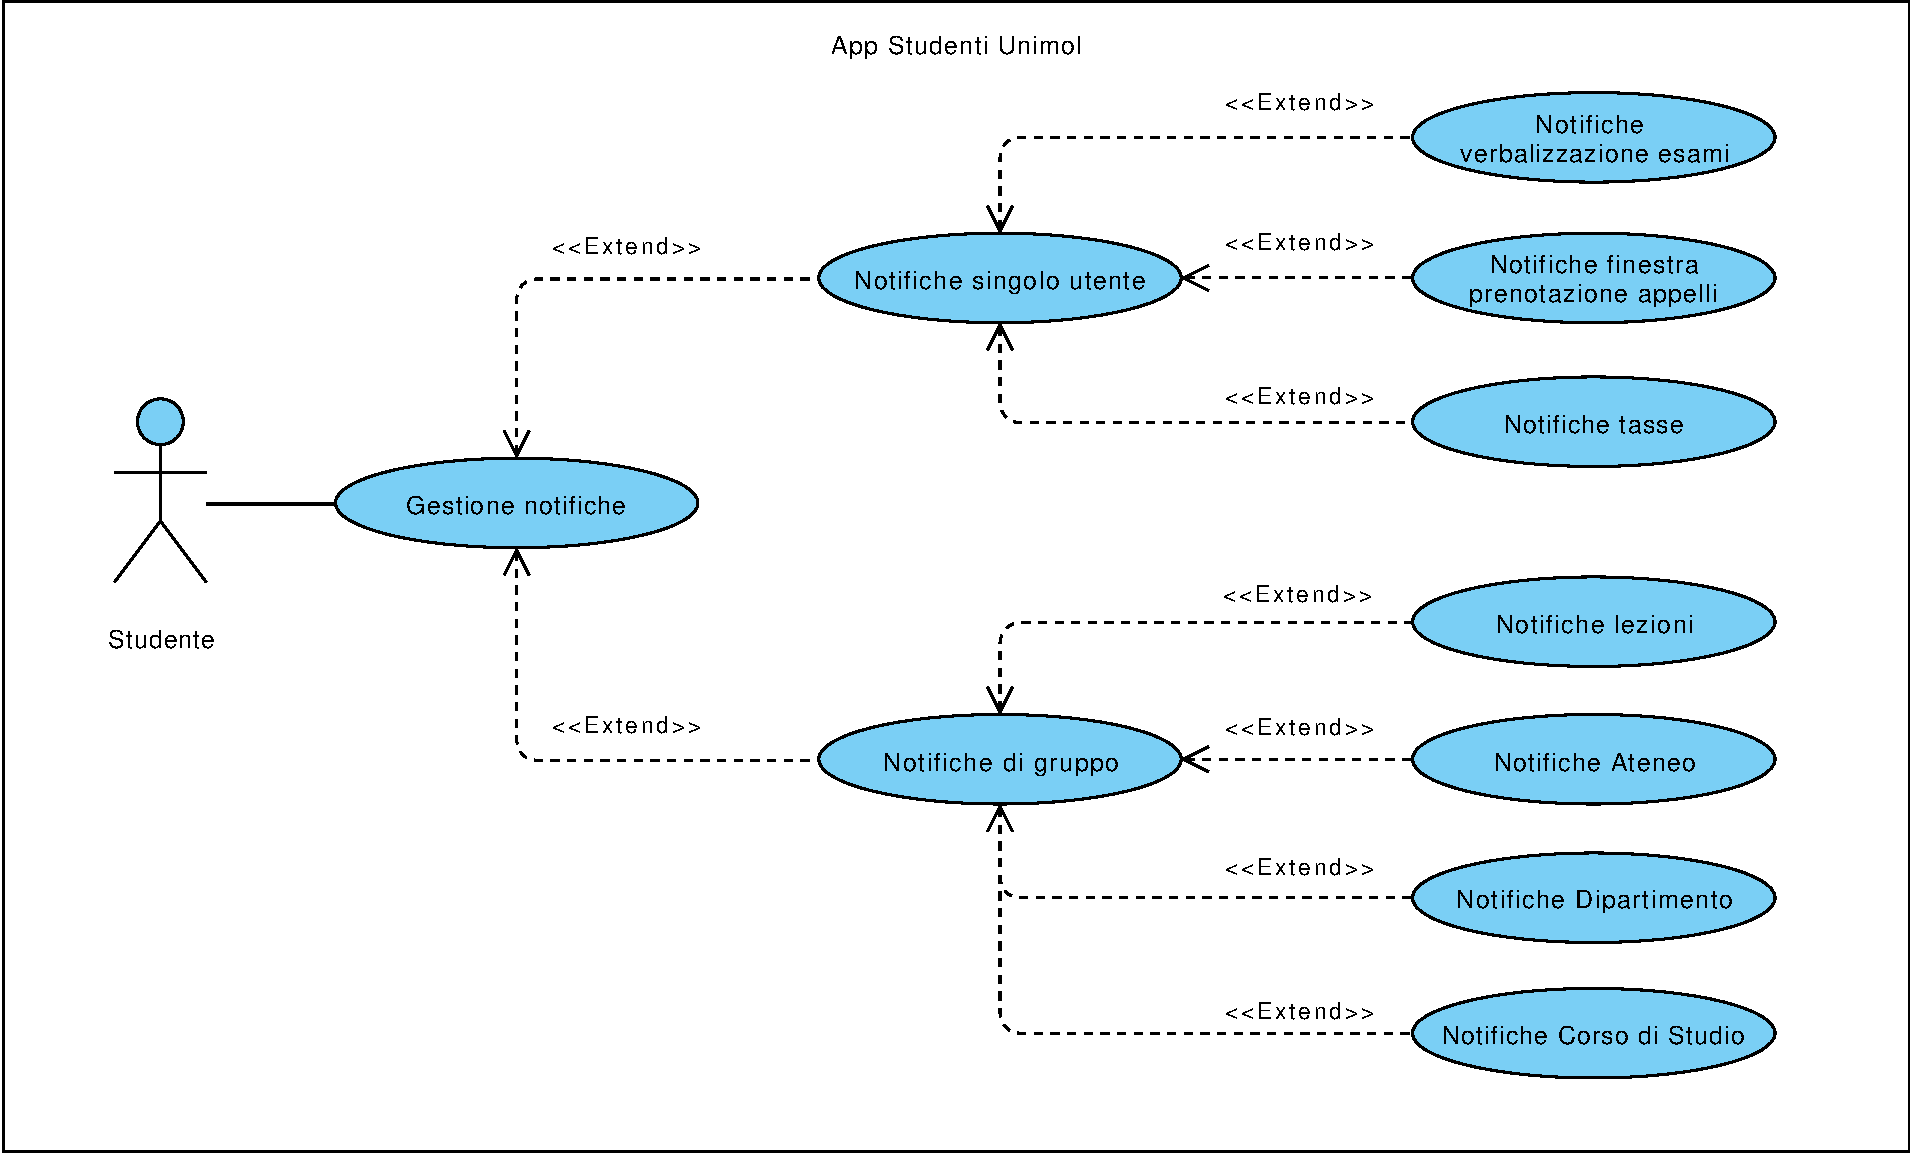
\includegraphics[width=\textwidth]{imgs/gruppo2/usecase-diagram-notifiche}
	\caption{Diagramma casi d'uso - Notifiche}
	\label{fig:diagr-casi-duso-notifiche}
\end{figure}

\section{Diagrammi di sequenza}

Diagramma di sequenza: Vedi Figura~\vref{fig:seq-diagr-notifiche}.

\begin{figure}
	\centering
	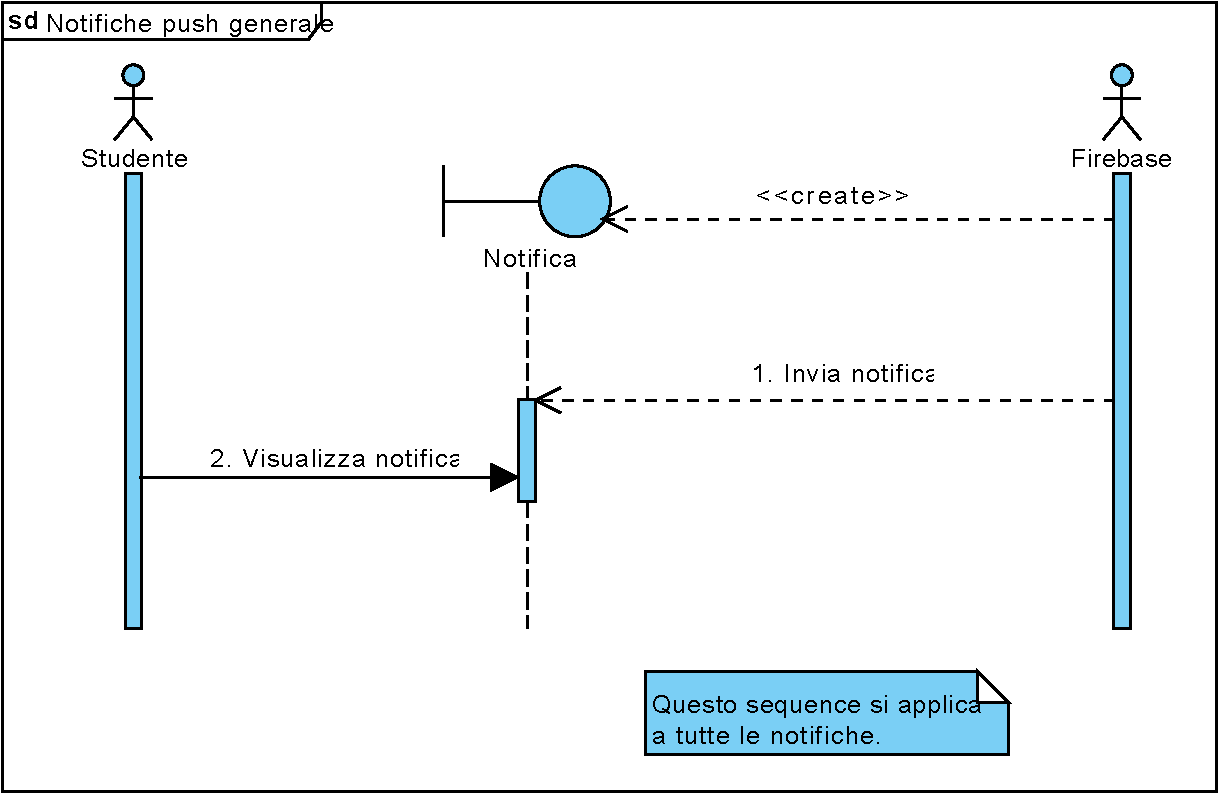
\includegraphics[width=0.85\textwidth]{imgs/gruppo2/sequence-notifiche}
	\caption{Sequence diagram - Notifiche}
	\label{fig:seq-diagr-notifiche}
\end{figure}

\section{Diagrammi delle attività}

Diagrammma per "Verbalizzazione esame": vedi Figura~\vref{fig:activity-notifiche-verbalizzazione-esame}.

Diagrammma per "Apertura finestra di prenotazione per l'appello d'esame": vedi Figura~\vref{fig:activity-notifiche-apertura-finestra-esame}.

Diagrammma per "Chiusura finestra di prenotazione per l'appello d'esame": vedi Figura~\vref{fig:activity-notifiche-chiusura-finestra-esame}.

Diagrammma per "Avviso tasse": vedi Figura~\vref{fig:activity-notifiche-avviso-tasse}.

Diagrammma per "Rinvio delle lezioni": vedi Figura~\vref{fig:activity-notifiche-rinvio-lezioni}.

Diagrammma per "Sospensione lezioni": vedi Figura~\vref{fig:activity-notifiche-sospensione-lezioni}.

Diagrammma per "Notizie dall'Ateneo": vedi Figura~\vref{fig:activity-notifiche-notizie-ateneo}.

Diagrammma per "Notizie dal Dipartimento": vedi Figura~\vref{fig:activity-notifiche-notizie-dipartimento}.

Diagrammma per "Notizie dal Corso di Studi": vedi Figura~\vref{fig:activity-notifiche-notizie-corso-di-studi}.

\begin{figure}
	\centering
	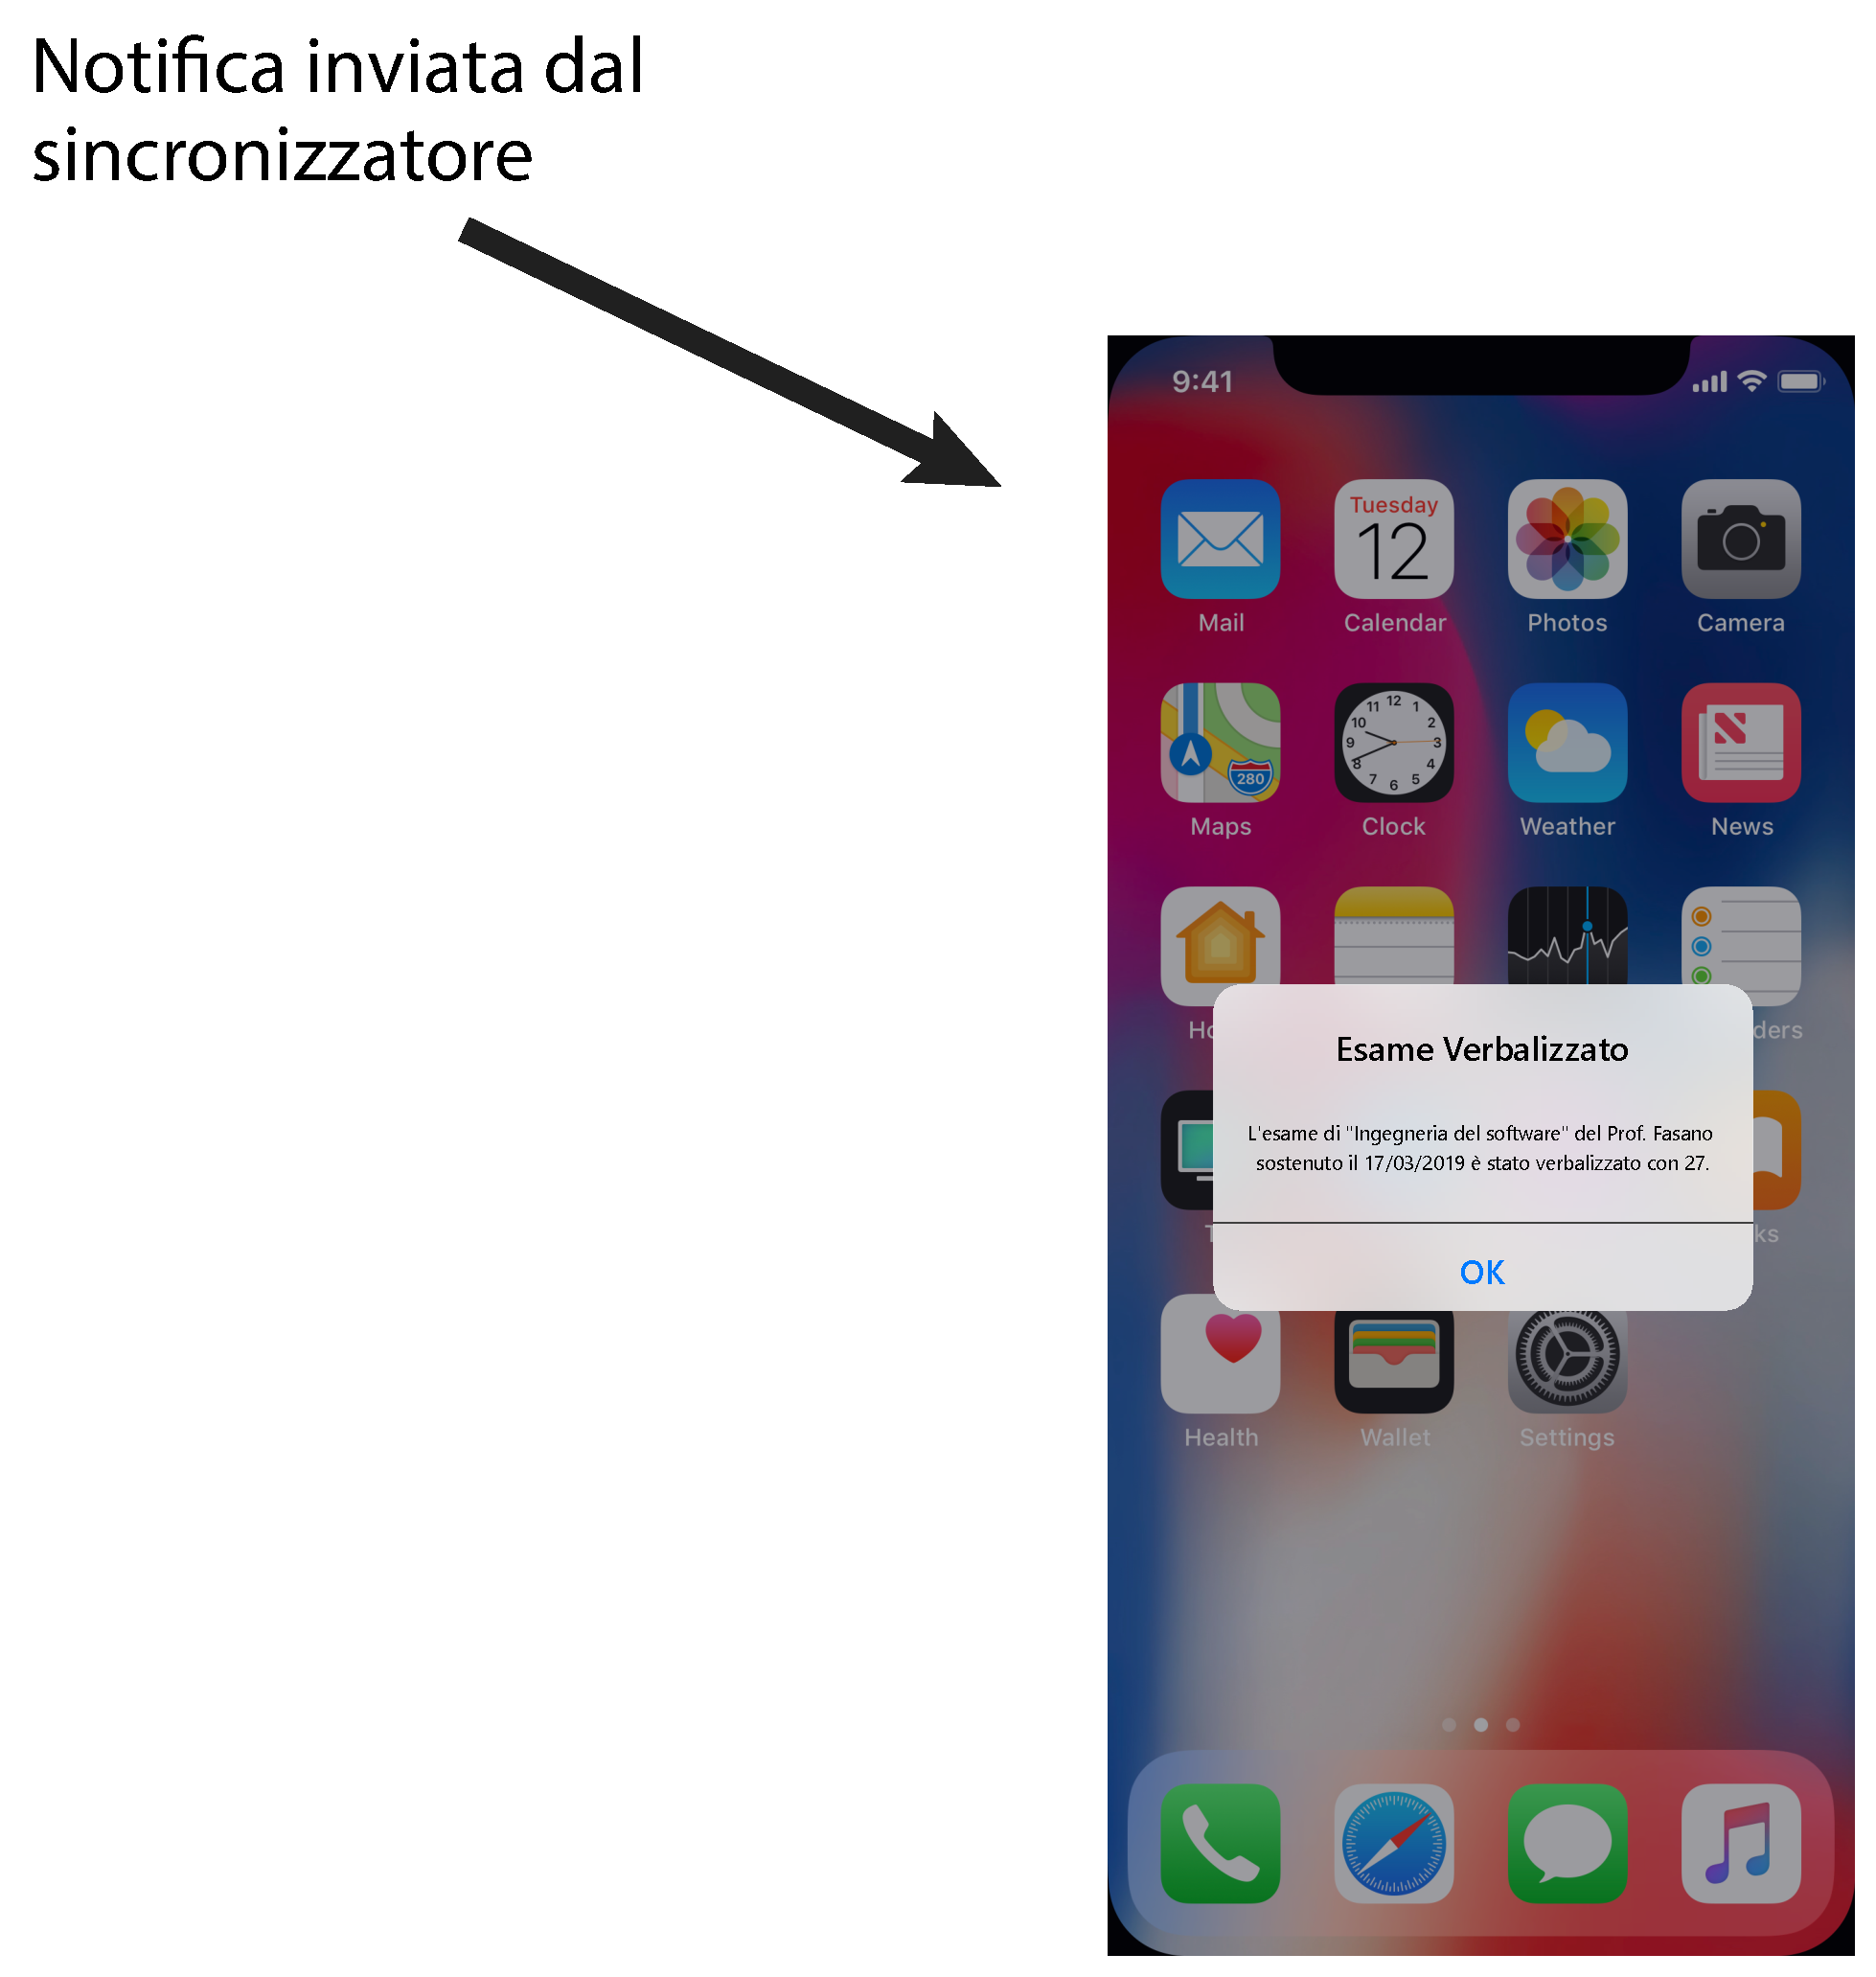
\includegraphics[width=0.67\textwidth]{imgs/gruppo2/activity-notifiche-verbalizzazione-esame}
	\caption{Activity - Verbalizzazione esame}
	\label{fig:activity-notifiche-verbalizzazione-esame}
\end{figure}

\begin{figure}
	\centering
	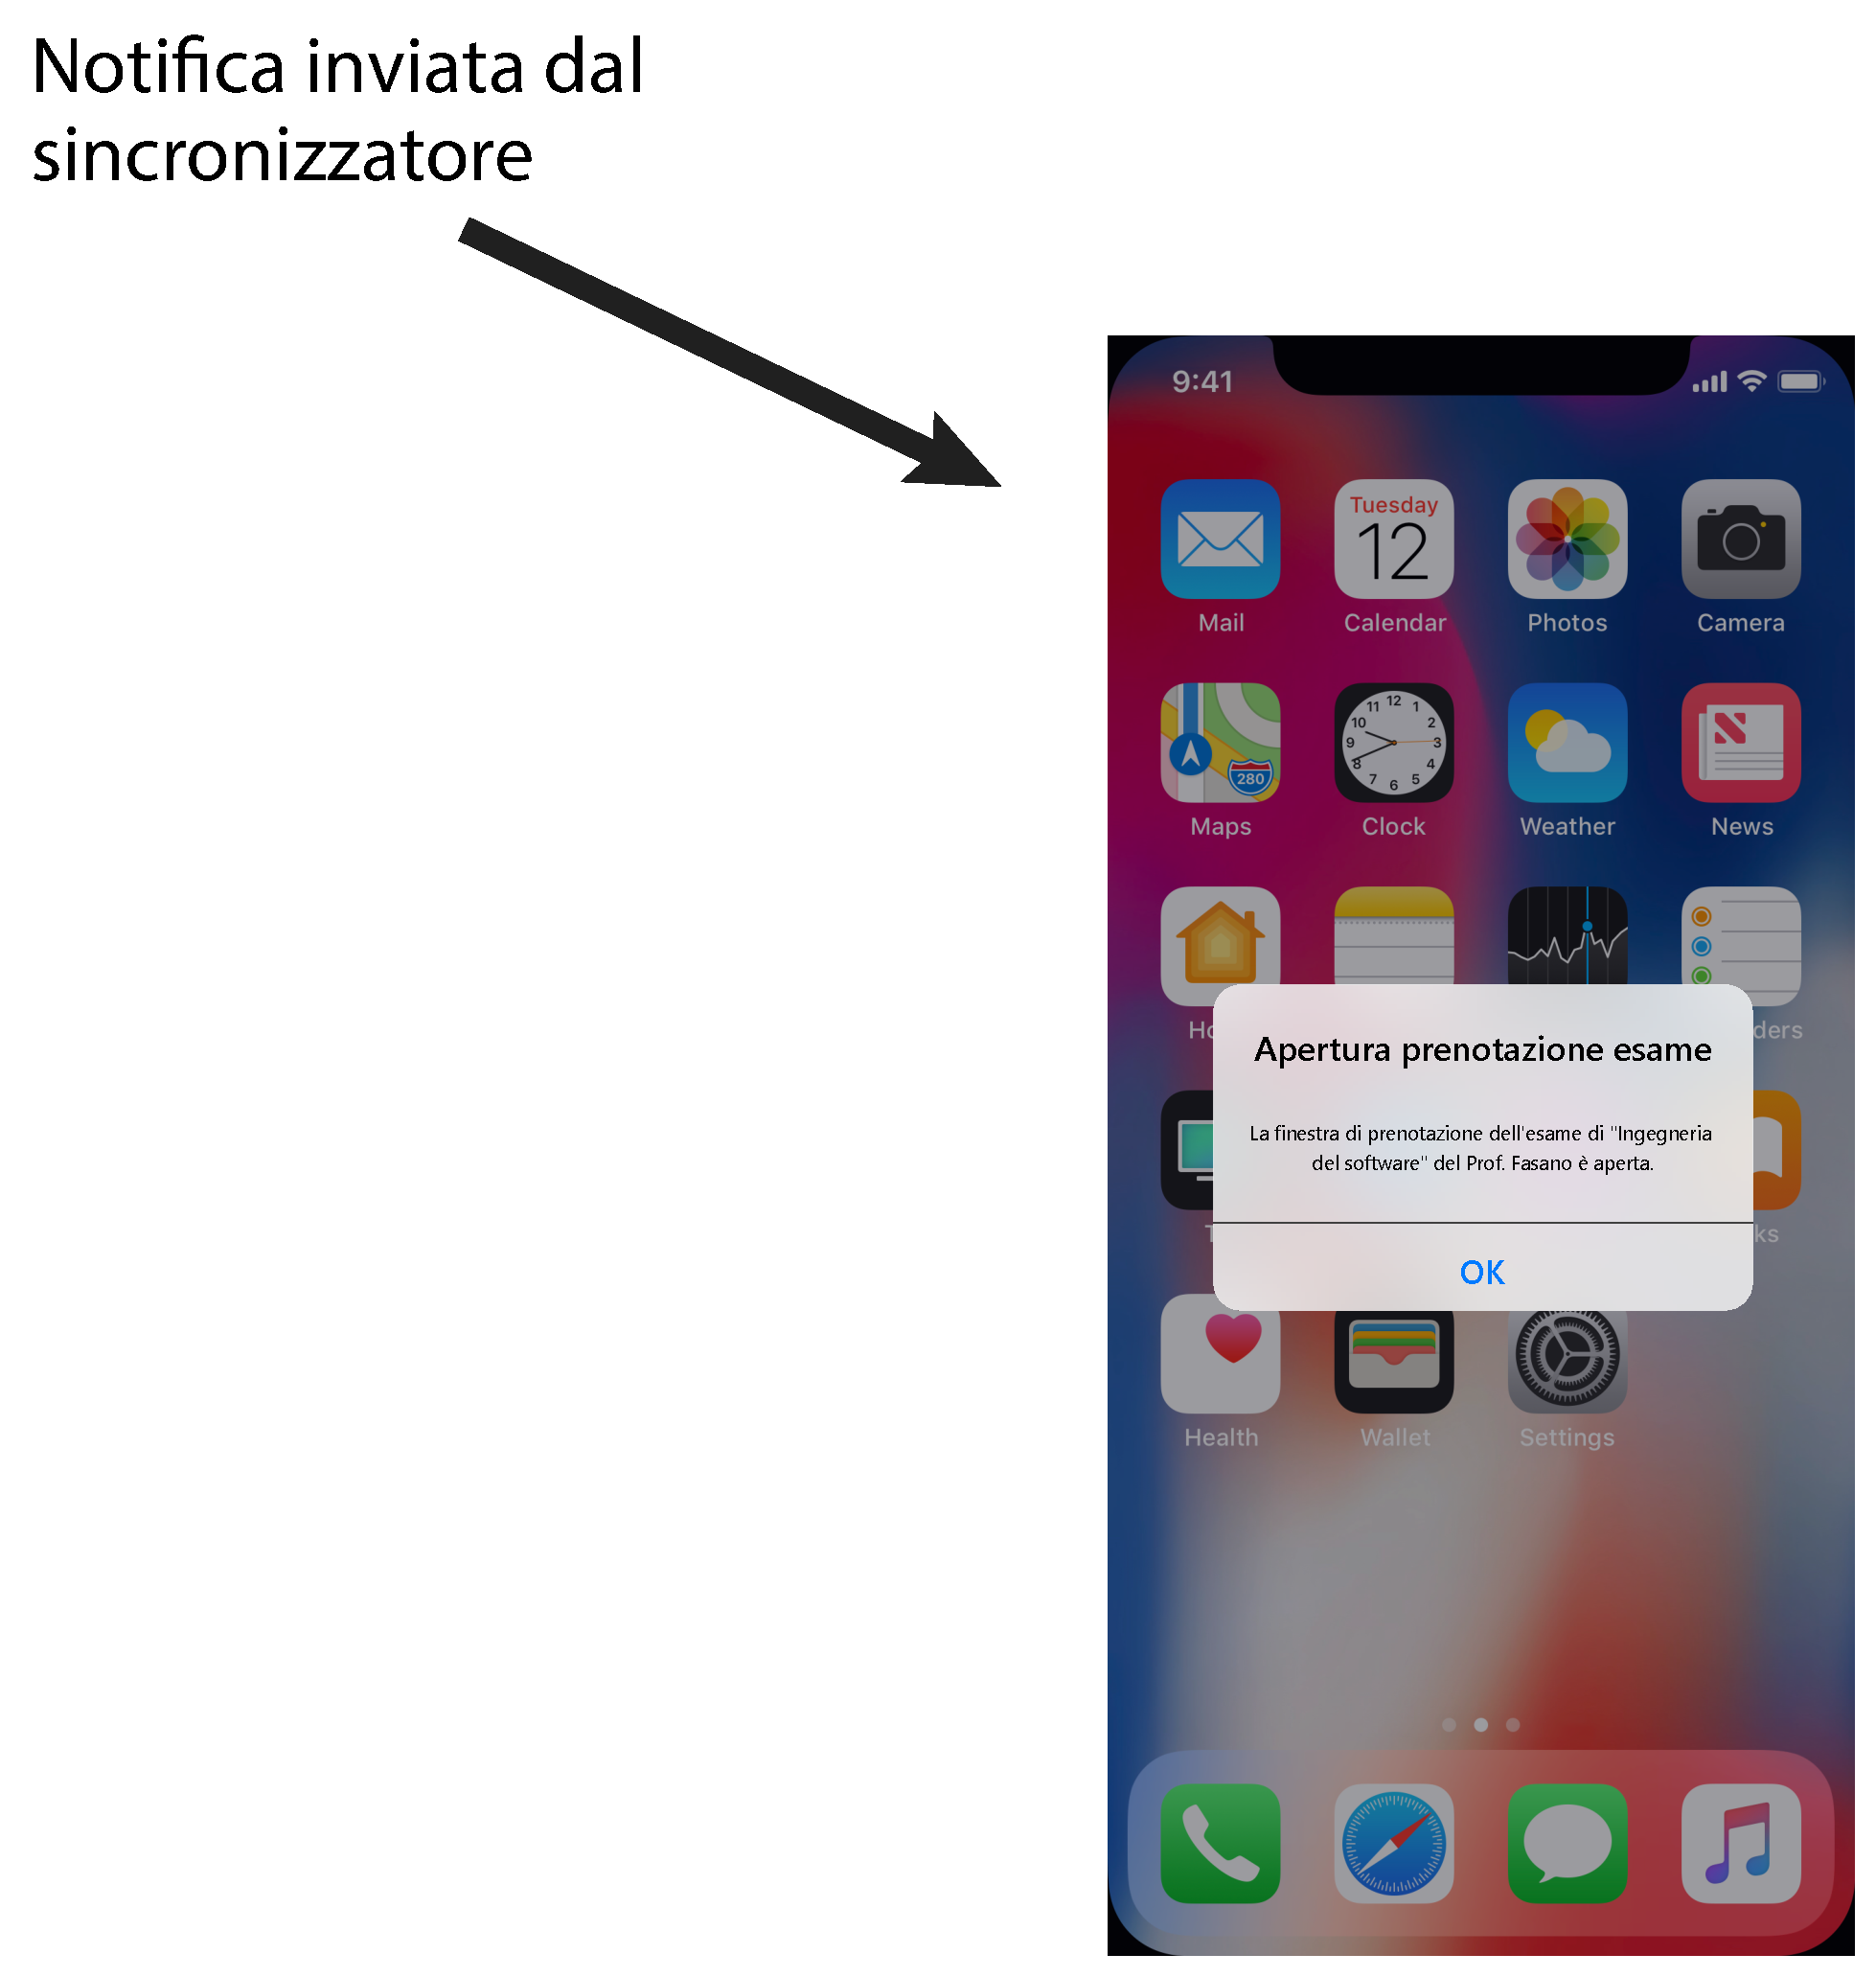
\includegraphics[width=0.67\textwidth]{imgs/gruppo2/activity-notifiche-apertura-prenotazione-esame}
	\caption{Activity - Apertura finestra di prenotazione per l'appello d'esame}
	\label{fig:activity-notifiche-apertura-finestra-esame}
\end{figure}

\begin{figure}
	\centering
	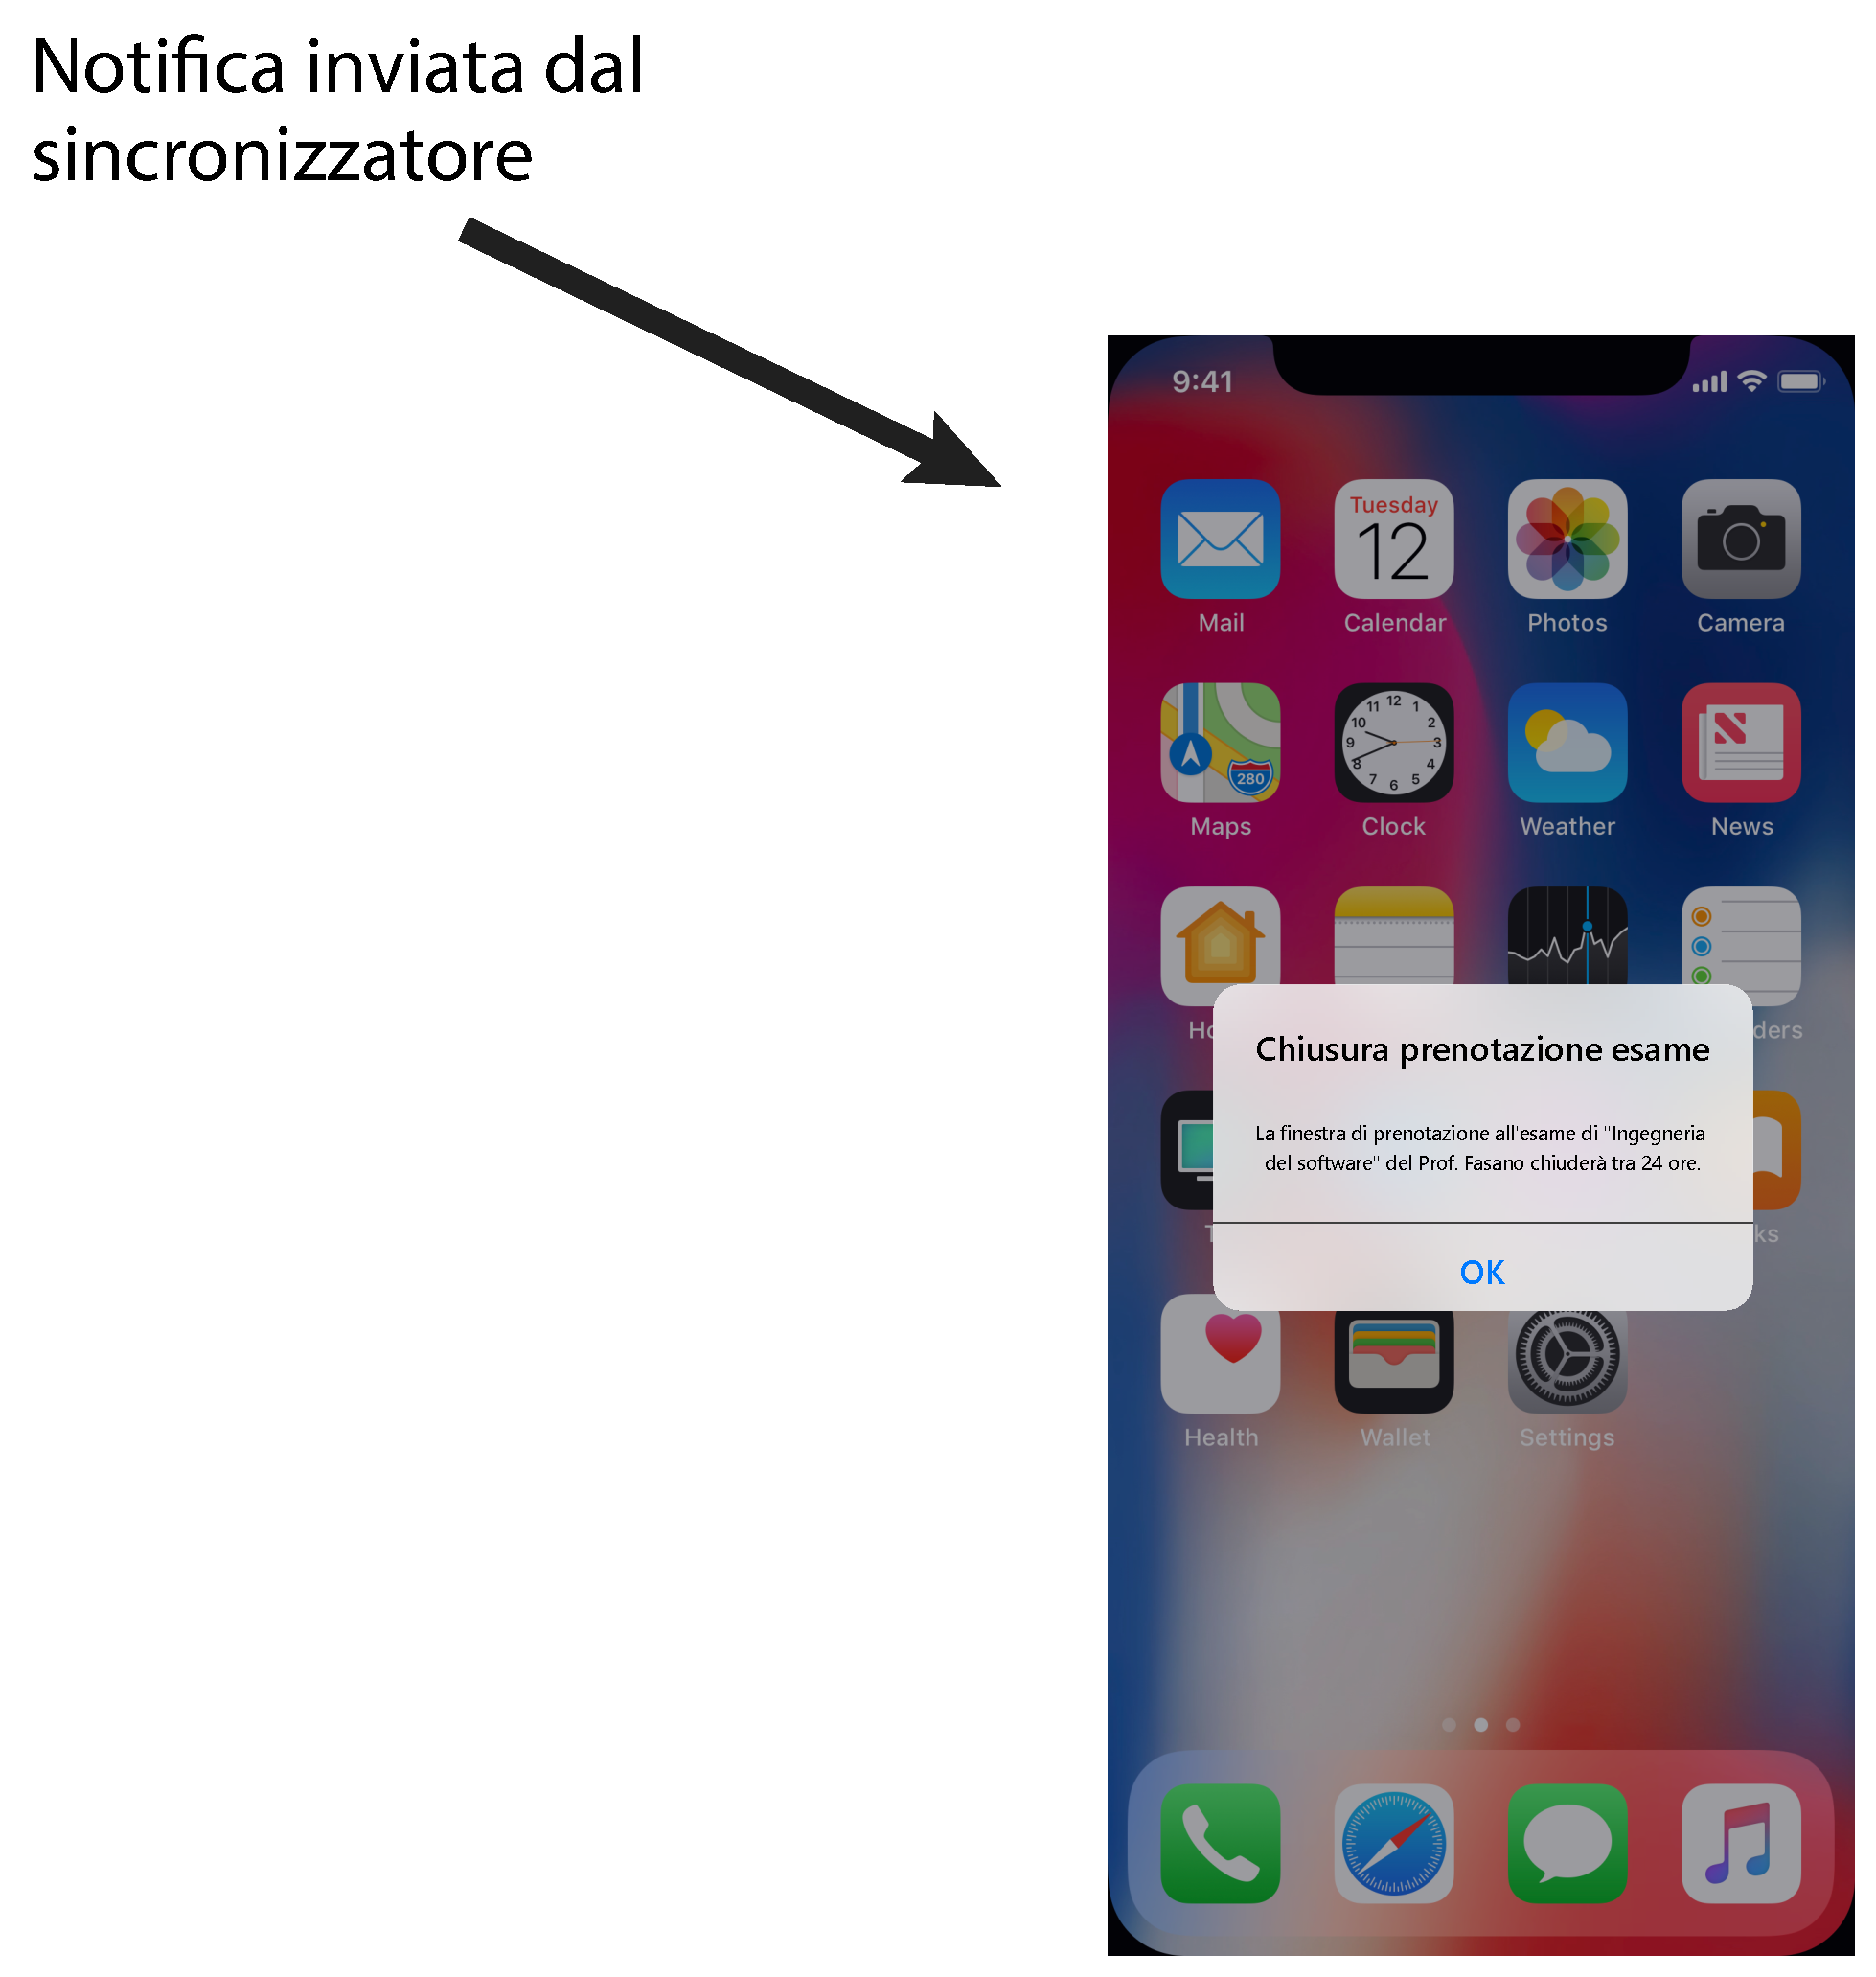
\includegraphics[width=0.67\textwidth]{imgs/gruppo2/activity-notifiche-chiusura-prenotazione-esame}
	\caption{Activity - Chiusura finestra di prenotazione per l'appello d'esame}
	\label{fig:activity-notifiche-chiusura-finestra-esame}
\end{figure}

\begin{figure}
	\centering
	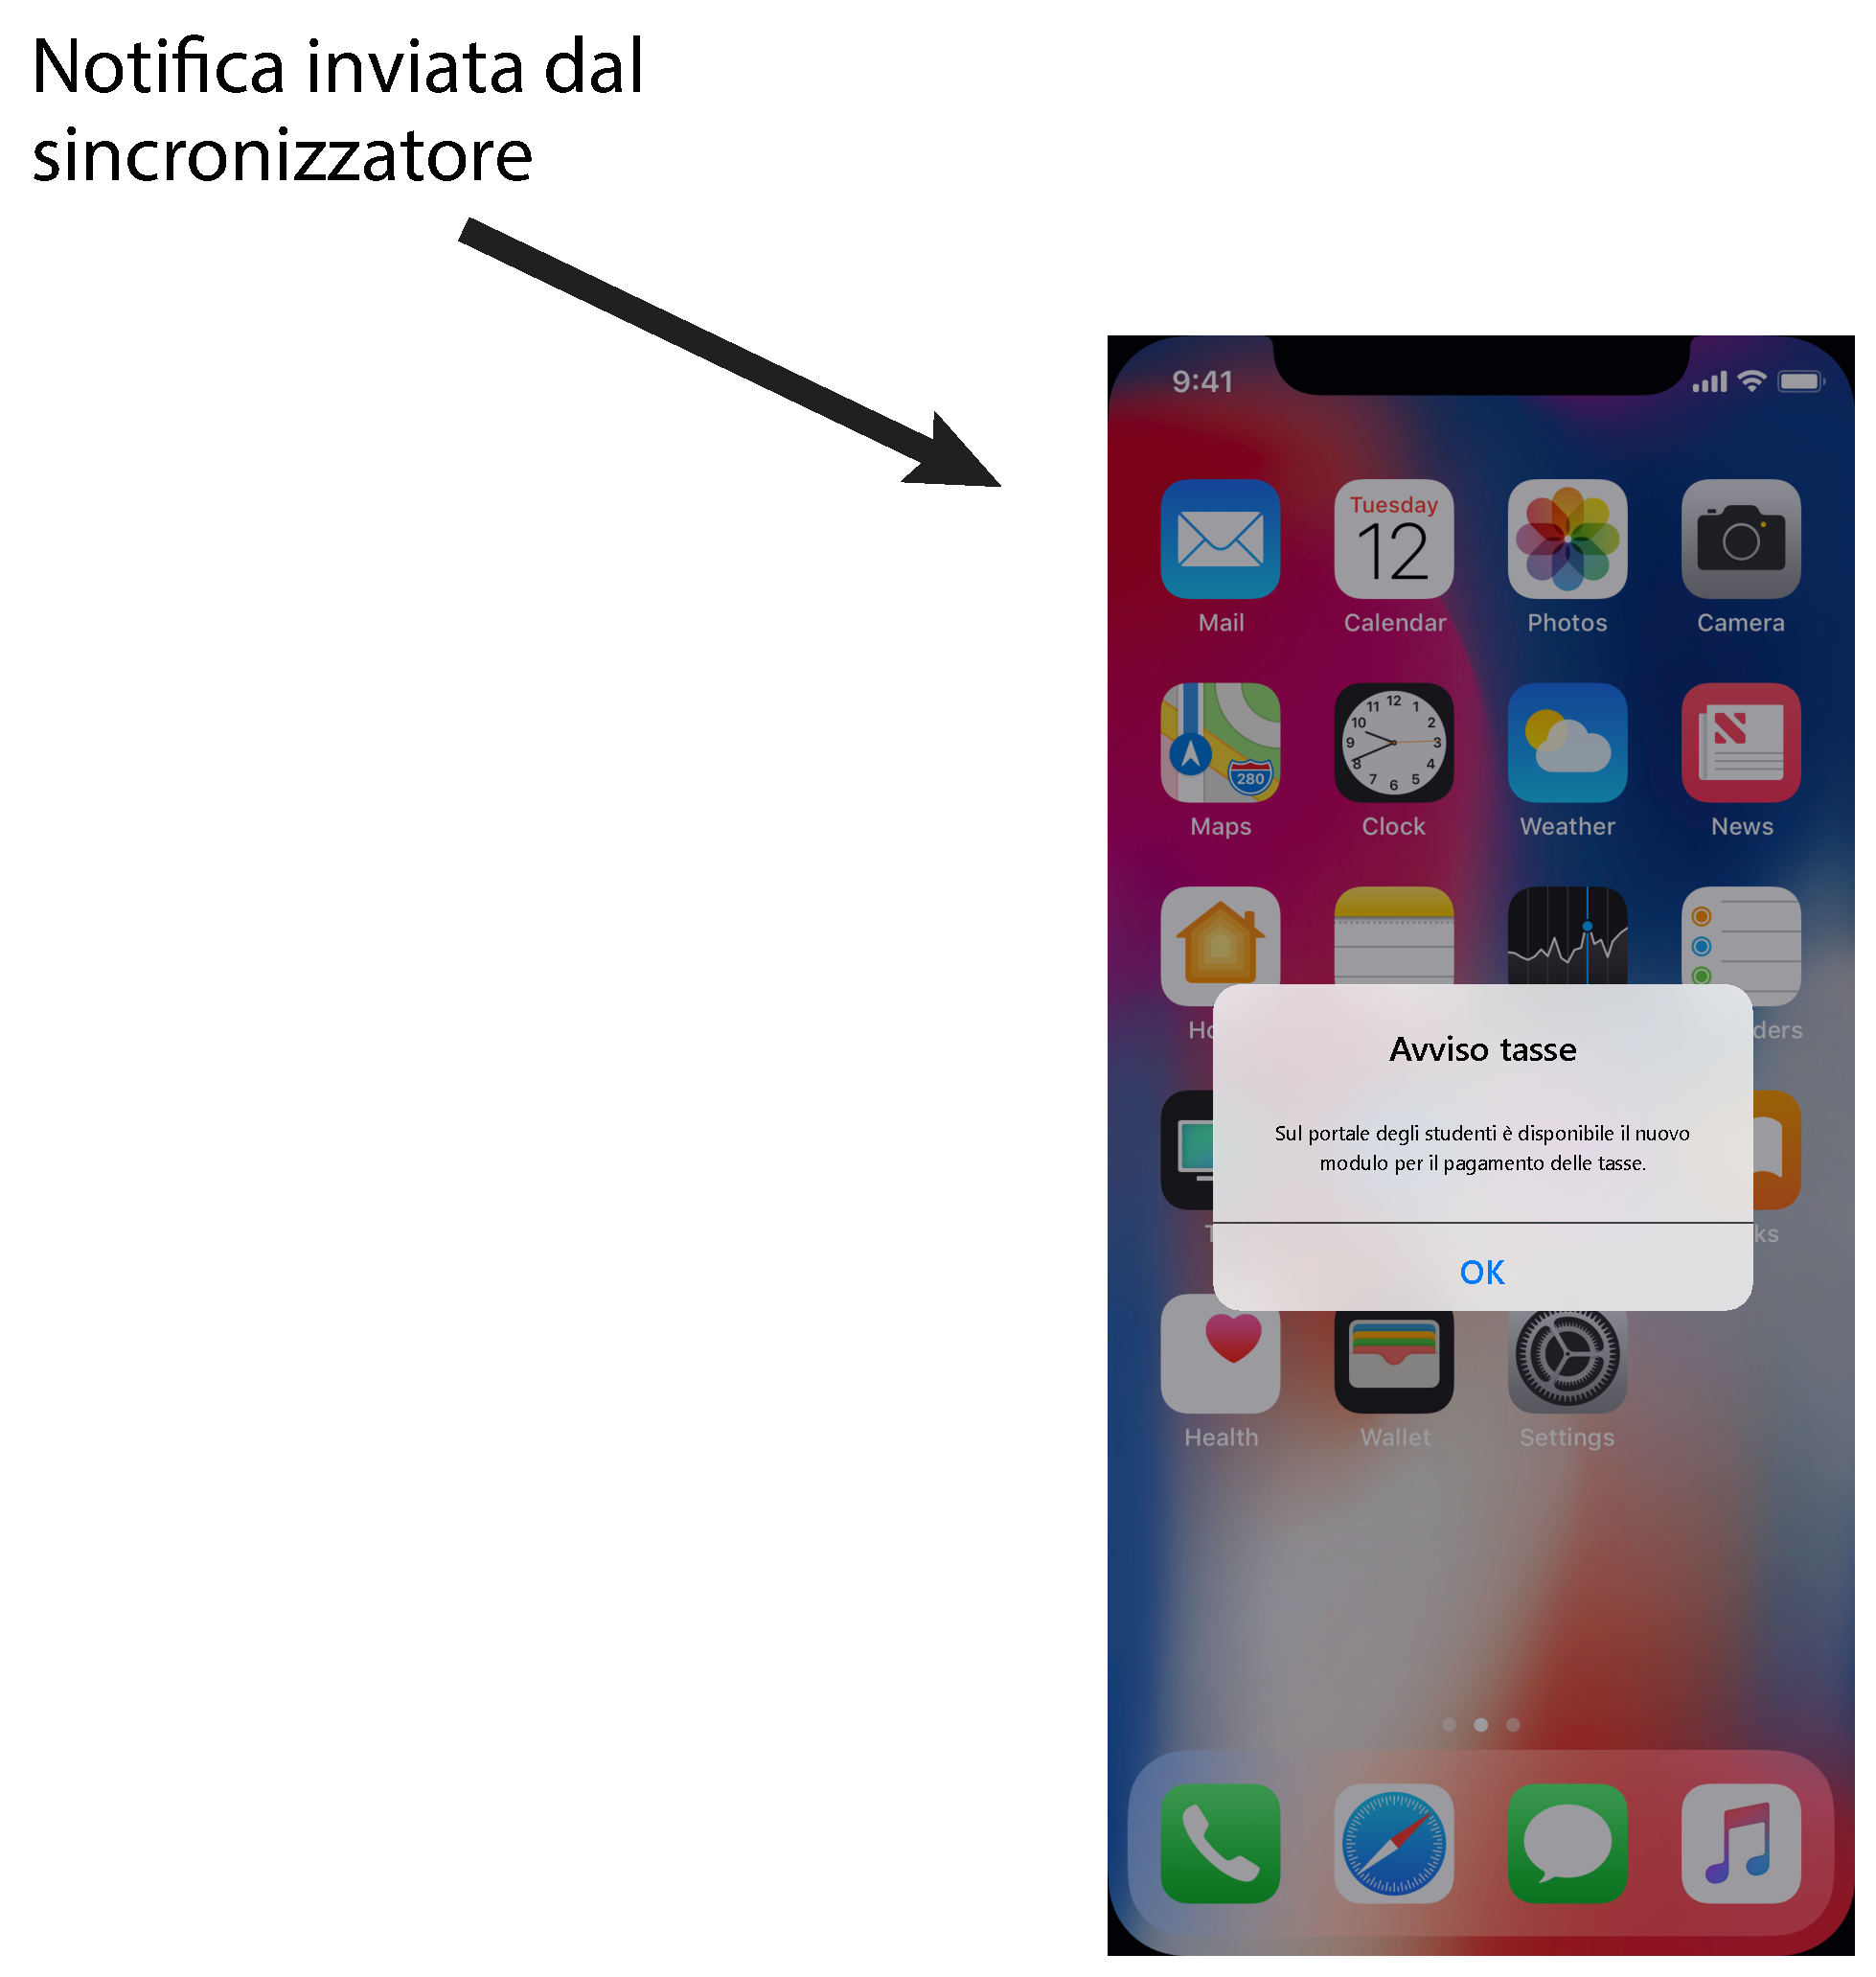
\includegraphics[width=0.67\textwidth]{imgs/gruppo2/activity-notifiche-avviso-tasse}
	\caption{Activity - Avviso tasse}
	\label{fig:activity-notifiche-avviso-tasse}
\end{figure}

\begin{figure}
	\centering
	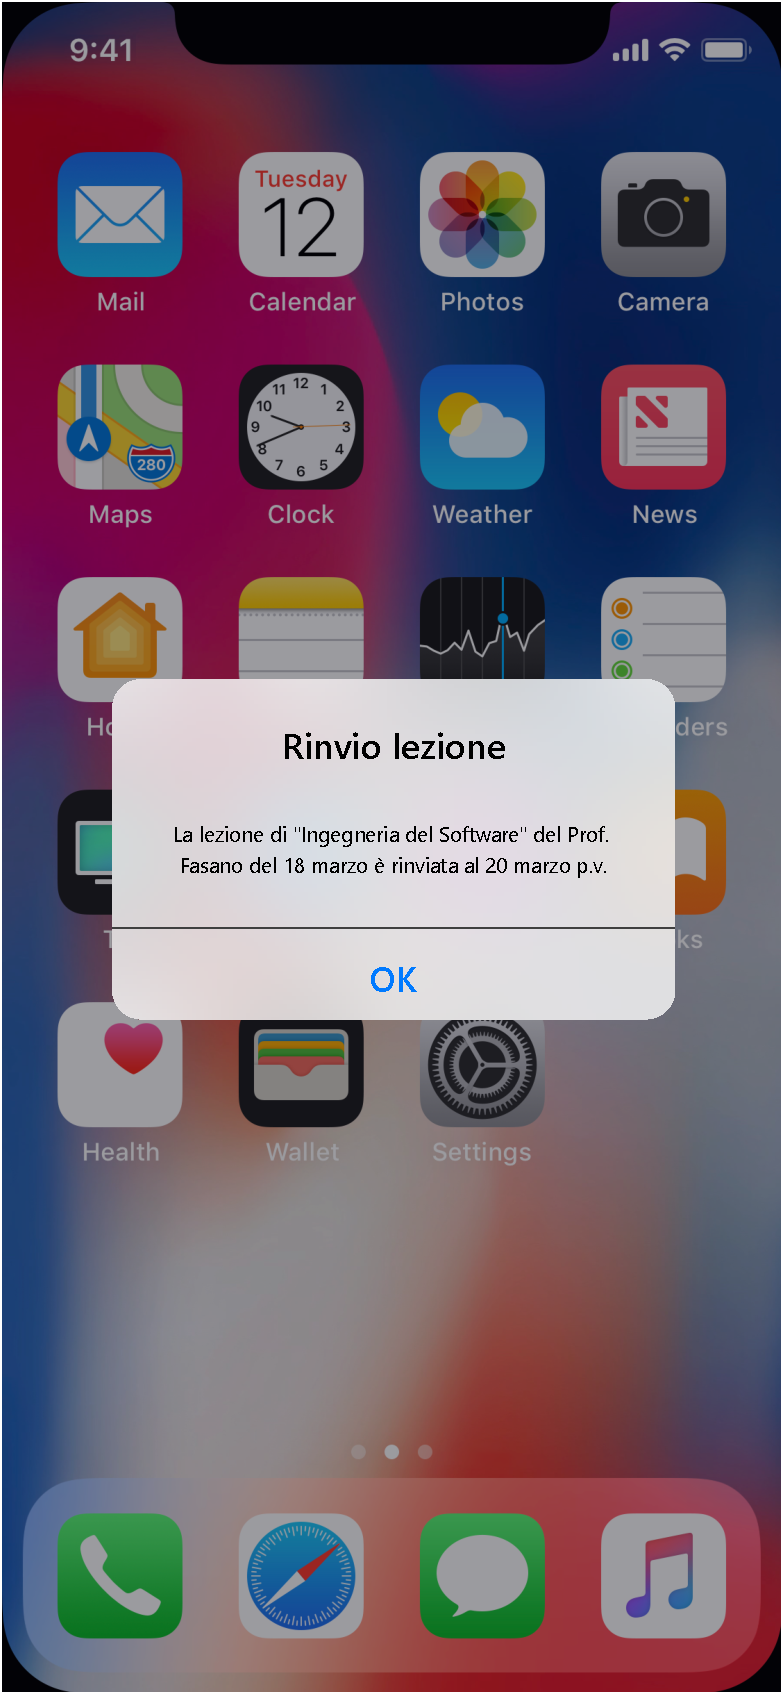
\includegraphics[width=0.67\textwidth]{imgs/gruppo2/activity-notifiche-rinvio-lezioni}
	\caption{Activity - Rinvio delle lezioni}
	\label{fig:activity-notifiche-rinvio-lezioni}
\end{figure}

\begin{figure}
	\centering
	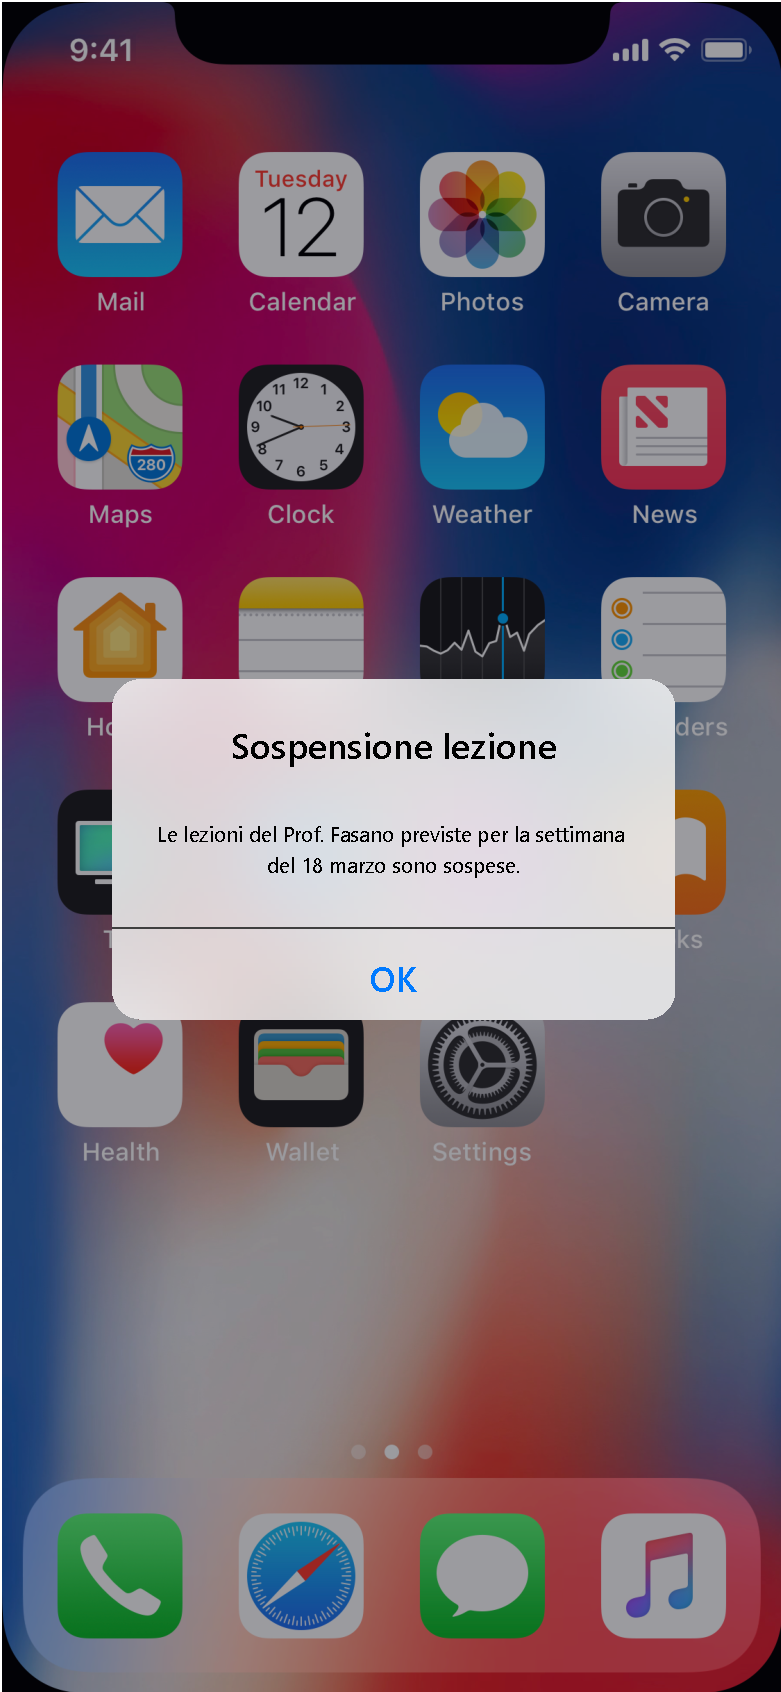
\includegraphics[width=0.67\textwidth]{imgs/gruppo2/activity-notifiche-sospensione-lezioni}
	\caption{Activity - Sospensione lezioni}
	\label{fig:activity-notifiche-sospensione-lezioni}
\end{figure}

\begin{figure}
	\centering
	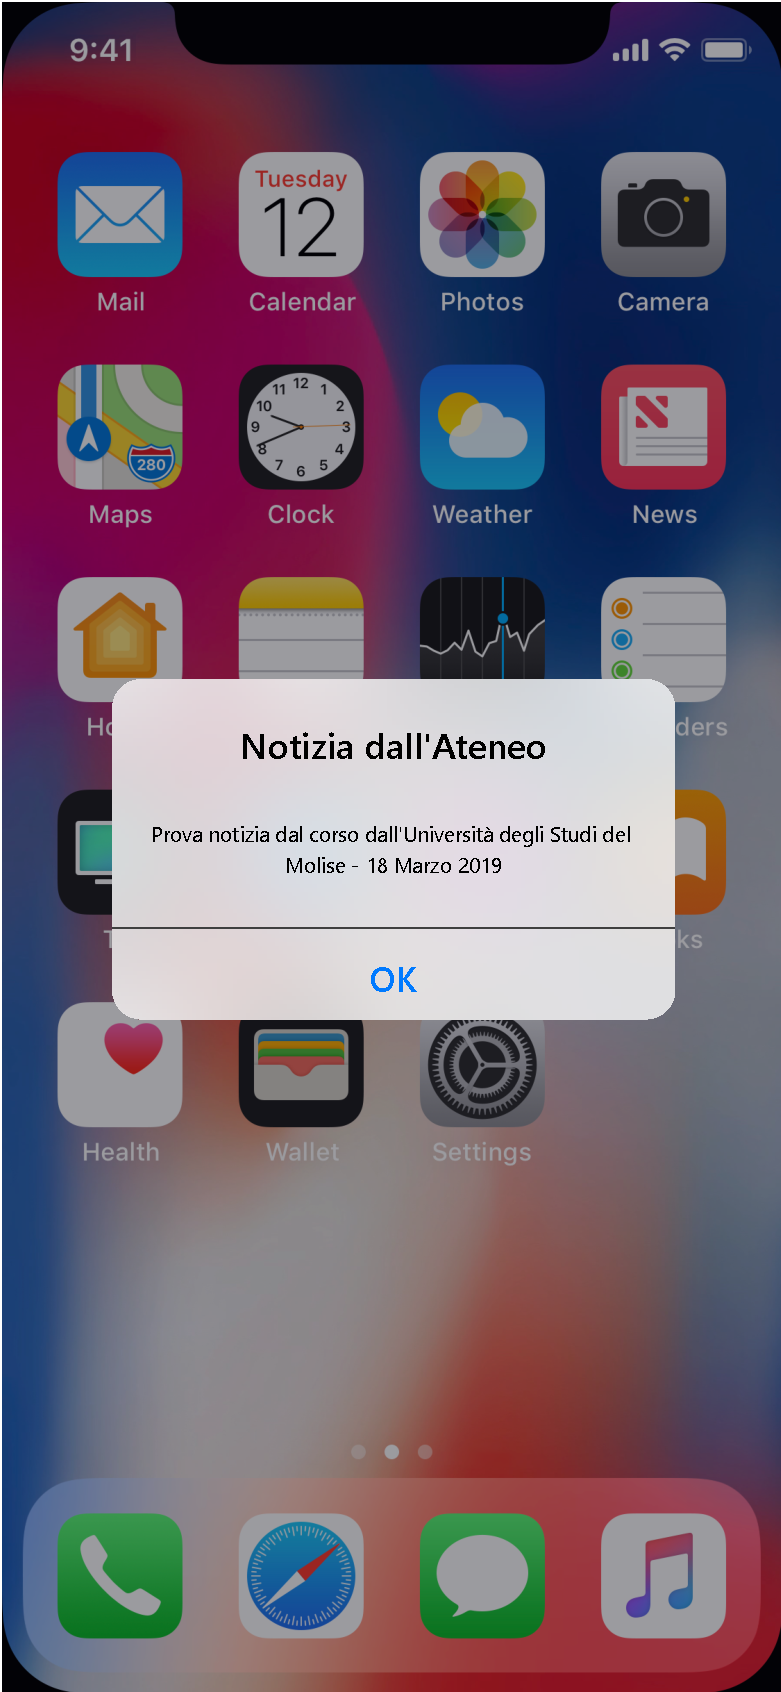
\includegraphics[width=0.67\textwidth]{imgs/gruppo2/activity-notifiche-notizie-ateneo}
	\caption{Activity - Notizie dall'Ateneo}
	\label{fig:activity-notifiche-notizie-ateneo}
\end{figure}

\begin{figure}
	\centering
	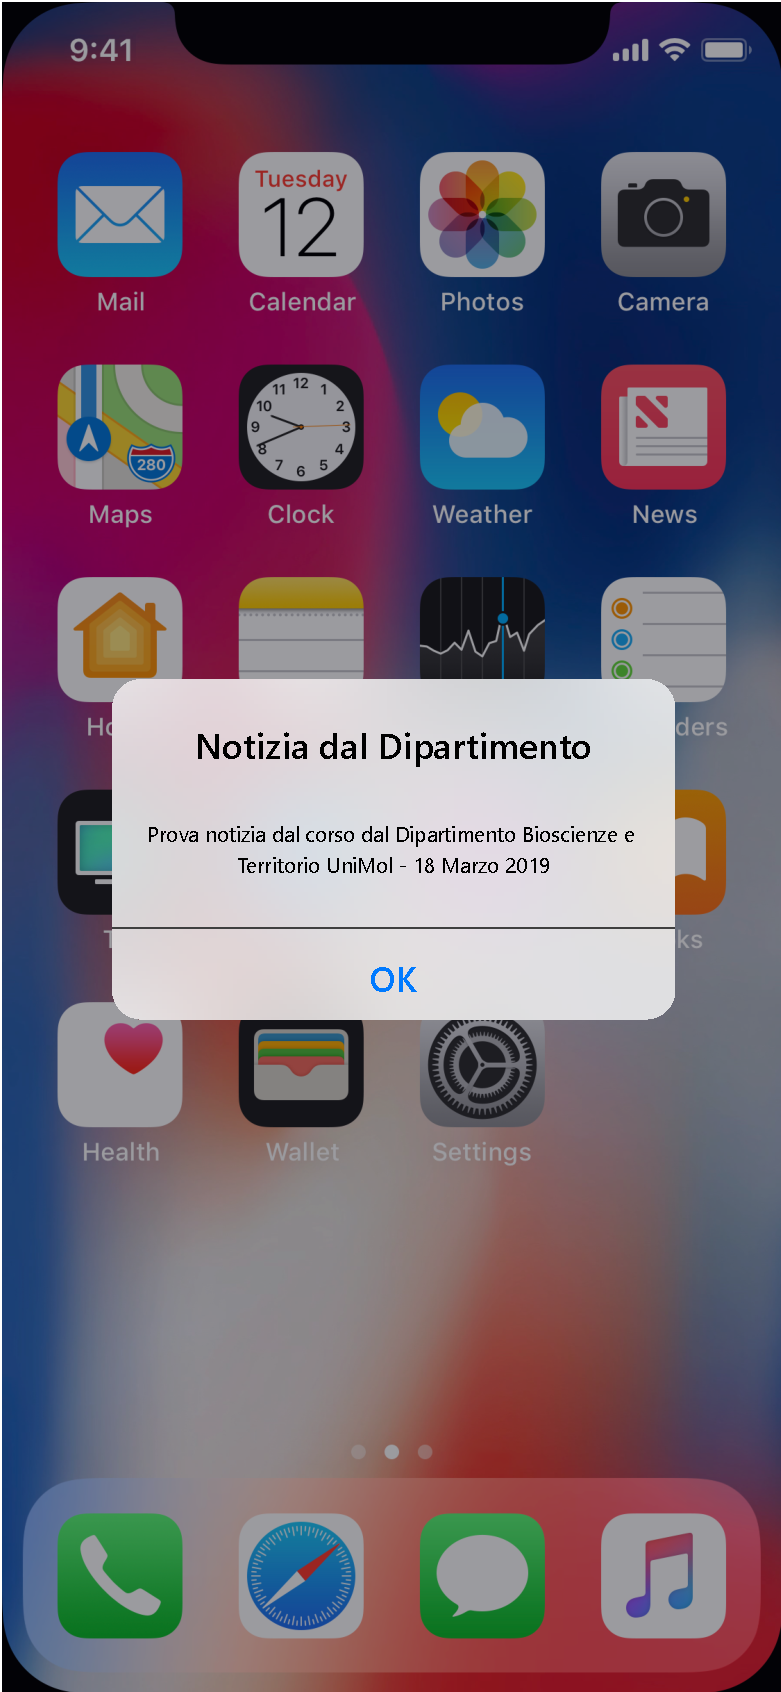
\includegraphics[width=0.67\textwidth]{imgs/gruppo2/activity-notifiche-notizie-dipartimento}
	\caption{Activity - Notizie dal Dipartimento}
	\label{fig:activity-notifiche-notizie-dipartimento}
\end{figure}

\begin{figure}
	\centering
	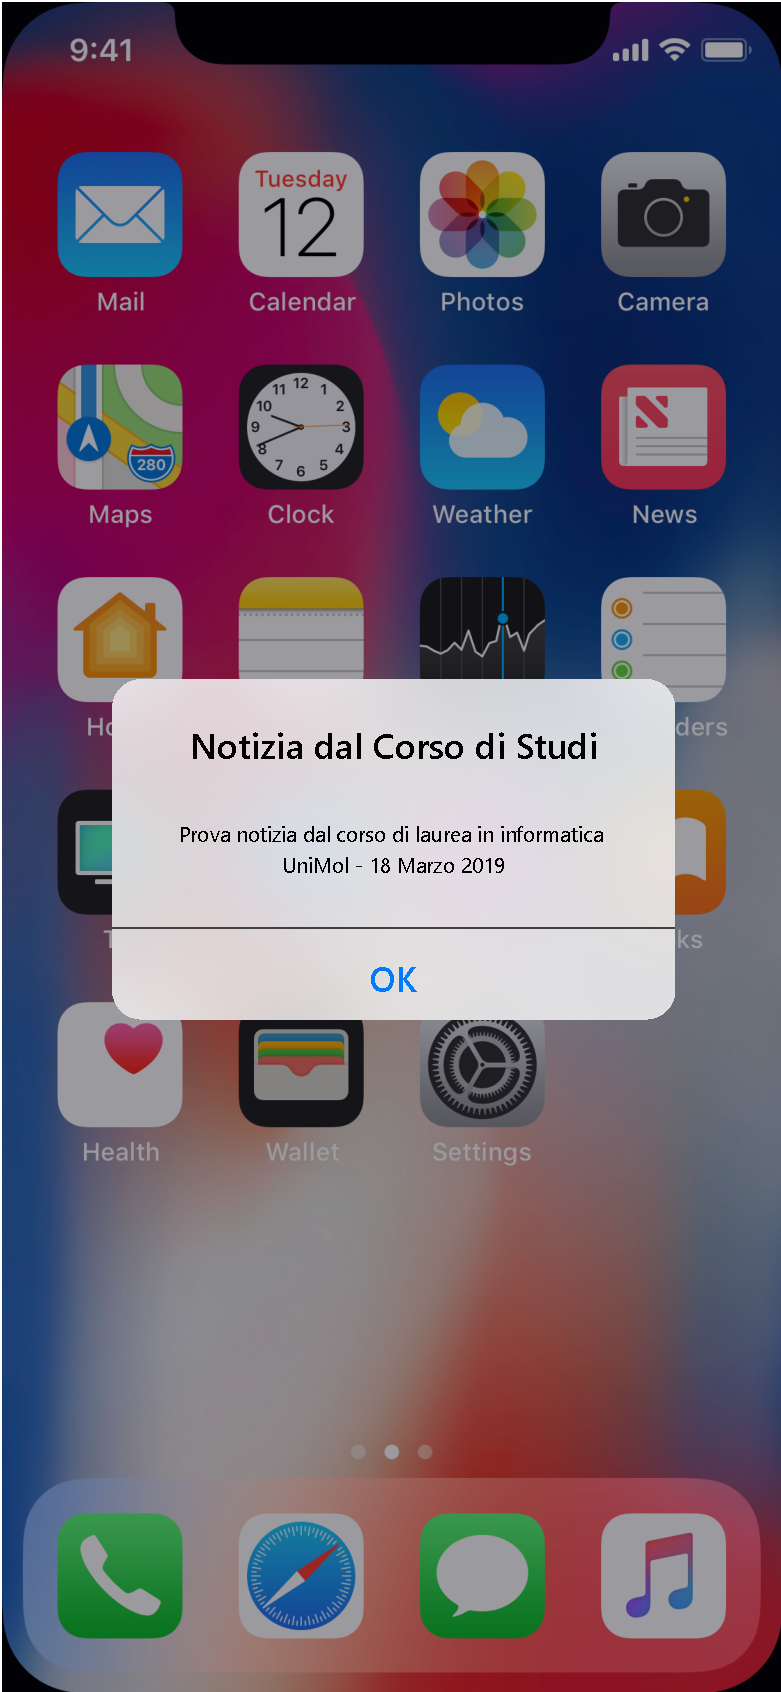
\includegraphics[width=0.67\textwidth]{imgs/gruppo2/activity-notifiche-notizie-corso-di-studi}
	\caption{Activity - Notizie dal Corso di Studi}
	\label{fig:activity-notifiche-notizie-corso-di-studi}
\end{figure}

\clearpage